\chapter{Concept}
\label{ch:concept}
This chapter introduces the functional and non-functional requirements of two 
applications - the container runtime and the benchmarking tool. 
In addition, architectural diagrams are provided and discussed. 
Example usage of both applications is shown.
This chapter also contains a thorough justification of the workloads deployed by the benchmarking tool as
well as the variables used to measure the performance of the sandboxed workloads.

\section{Container runtime}
The container runtime is the component responsible for wrapping a user-defined binary 
in a sandbox. It will be used by the benchmarking tool to wrap workloads in sandboxes.

\subsection{Functional requirements}
The Open Containers Initiative standardises the operations \cite{oci-runtime-operations} that 
a container runtime needs to support.

\begin{enumerate}[i]
\item The container runtime must provide clients with state information for a container
given its unique identifier. 
\label{requirements:container-runtime/1}
\item The container runtime must provide clients with the ability to create a new container. 
Users must supply the runtime with a unique identifier for the container and a path to a 
container bundle. The latter consists of a root filesystem and a configuration file that 
defines, amongst other things, the path to the user-defined binary and the set of namespaces
it will reside in.
\label{requirements:container-runtime/2}
\item The container runtime must provide clients with the ability to start a container. 
Users must provide the unique identifier of the container to start. 
This operation must execute the user-defined binary in the sandboxed environment.
\label{requirements:container-runtime/3}
\item The container runtime must allow users to kill the container process.
Users are required to provide the unique identifier of the container and the signal to be sent 
to the container.
\label{requirements:container-runtime/4}
\item The container runtime must allow users to delete the container.
The delete operation must remove all resources allocated in (\ref{requirements:container-runtime/2})
\label{requirements:container-runtime/5}
\item The container runtime must allow external applications to hook into well-defined points 
of a container's lifecycle.
\label{requirements:container-runtime/6}
\end{enumerate}

It is important to note that the container runtime's only responsibility is to sandbox processes. 
An external application, such as the benchmarking tool discussed later, 
must have the ability to interact with the runtime for the purpose of configuring 
the sandboxed environment. This includes operations such as creating network topologies that interconnect 
different containers or allocating shared filesystems. From this, requirement 
(\ref{requirements:container-runtime/6}) has been derived. 

\subsection{Non-functional requirements}
All requirements specified in this section are ranked in order of importance. 
\begin{enumerate}[i]
\item The container runtime must not pollute or damage the host system via its operation.
The runtime manages sensible resources, such as mount points and devices. It must in no way 
cause side effects on the host, leading to operational failure. This is also an important factor 
for allowing reproducibility of the work. Users must be able to use the runtime without fear of 
damaging their system. 
\label{requirements:non-functional/container-runtime/1}
\item The container runtime must support unprivileged containers, i.e containers that run without 
root privileges on the host system. This is in and of itself a functional requirement for running 
containers in multitenant environments. 
\label{requirements:non-functional/container-runtime/2} 
\item The container runtime must be implemented in a programming language with manual memory management.
Satisfying this requirement will ensure that future work aimed at measuring container boot times 
will not be hindered by unpredictable perturbations introduced by a garbage collector.
\label{requirements:non-functional/container-runtime/3}
\item The container runtime must consist of a library component and an executable component. 
This will allow users to implement their own abstractions on top of the library for other research-related 
purposes. 
\end{enumerate}

\subsection{Architecture}
\begin{figure}[H]
    \centering
    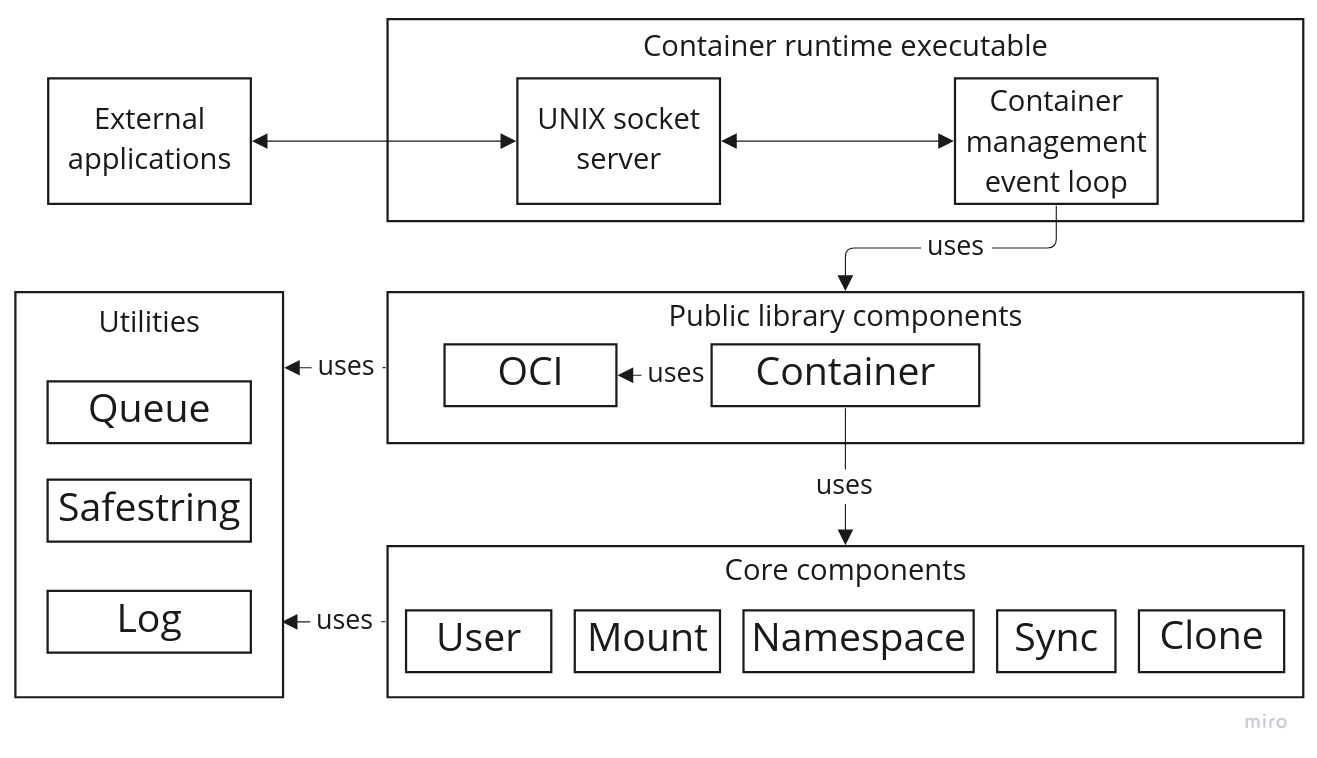
\includegraphics[width=0.55\textwidth]{images/concept/runtime-arch-overview.jpg}
    \caption{High-level overview of the runtime architecture}
    \label{images:concept/runtime-arch-overview.jpg}
\end{figure}
The architecture of the runtime is shown in Figure \ref{images:concept/runtime-arch-overview.jpg}.
It consists of a library and an executable that uses it to provide container 
management services to external applications. The library is split into three parts - utilities,
core components and public components. 

The utilities provide common data structures such as 
linked lists and queues. They also contain procedures for safe string manipulation, a logger,
and a multitude of helper macros that enable the safe management of resources such as file descriptors 
and heap memory. The core components directly interface with the kernel. 
They are responsible for configuring the container, 
i.e the execution environment of the user-defined application. On top, the public library 
components use the core components to provide a 
simple interface for creating, starting, killing and deleting containers. A container 
is represented as an opaque pointer and is only allowed to be accessed through library functions.

The runtime executable uses the container component to create and manage a single container.
It consists of an event loop that monitors state changes of the container and reaps the process 
when it exits. In addition, it polls a signal file descriptor for itself. When the user desides 
to kill the runtime executable, the same signal is propagated to the container, the container 
is killed, and all resources it allocated are deleted accordingly. 

When a process is detached into a new user namespace, it's real user identifier is replaced by the kernel 
with the overflow identifier, also known as the \textit{nobody} user, which has no access to 
file objects that are not world readable and writable. 
For this reason, the container runtime must map a range of user identifers from the root user namespace 
into a range of user identifiers in the user namespace of the process. The user component in Figure 
\ref{images:concept/runtime-arch-overview.jpg} is responsible for this functionality. 

\begin{figure}[H]
    \centering
    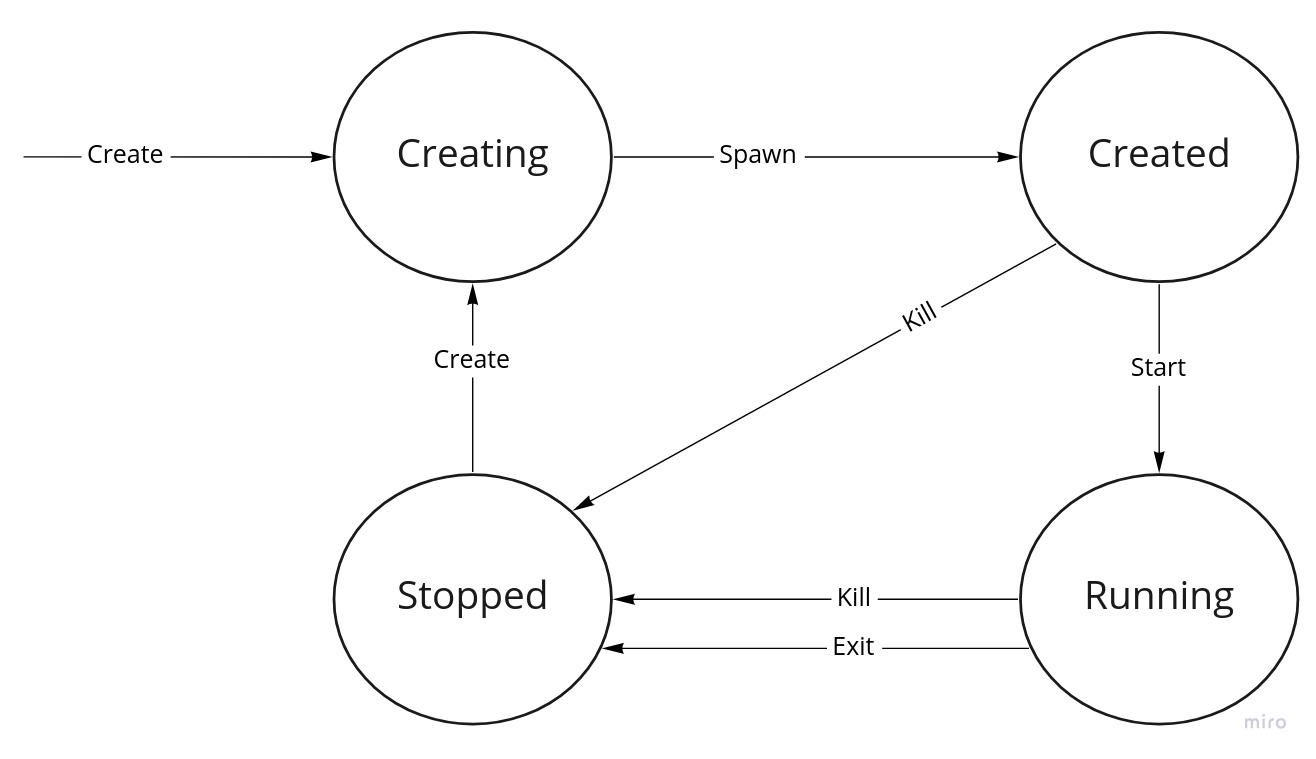
\includegraphics[width=0.5\textwidth]{images/concept/container-state-diagram.jpg}
    \caption{State transition diagram of container states. Every state transition is triggered by an operation, whose name is 
    specified in the arrow.}
    \label{images:concept/container-state-diagram.jpg}
\end{figure}

%\begin{table}[h!]
%    \centering
%    \begin{tabular}{ |m{3.5cm}|m{3.5cm}|m{20em}| }
%        \hline
%        Lifecycle Checkpoint & Request & Description \\
%        \hline
%        Runtime Creation & \verb|EVENT_RT_CREATE| & The container instructs the runtime to execute the runtime creation hooks on the host \\
%        \hline 
%        Container Creation & \verb|EVENT_CONT_CREATE| & The runtime instructs the container to execute the container creation hooks inside the container environment, after the runtime has been created \\
%        \hline 
%        Container Starting & \verb|EVENT_CONT_START| & The runtime instructs the container to execute the container start hooks inside the container environment, right before the user-defined binary is executed \\
%        \hline 
%        Container Started & \verb|EVENT_CONT_STARTED| & The container instructs the runtime to execute the container post-start hooks inside the runtime environment, right after the user-defined binary is executed \\
%        \hline 
%    \end{tabular}
%    \caption{Table of requests}
%    \label{table:concept/container-runtime/architecture/events}
%\end{table}

Every container has a dedicated root filesystem with its own set of device nodes,
pseudo filesystems, applications and libraries. The mount component in Figure \ref{images:concept/runtime-arch-overview.jpg}
atomically changes the container's root mount to a user-defined directory that holds its new root file system.
It then creates private mount points for all necessary pseudo filesystems, e.g \verb|proc|, \verb|sys|, and \verb|mqueue|. 
In addition, this component creates private device nodes for the container such as \verb|/dev/null| and \verb|/dev/urandom|.

The namespace component simply wraps some of the namespace system calls and provides a 
mechanism to enumerate a contiguous sequence of namespaces.

The clone component wraps the raw \verb|clone3()| system call and the \verb|glibc| wrapper 
into a portable (at least for \verb|x86_64| and \verb|aarch64|) set of functions.

The Open Containers Initiative (OCI) component is responsible for parsing a JSON configuration 
file that defines the container's execution environment. Code snippet \ref{code:oci-config.json} 
is an example of such a file. In addition, this component provides a mechanism for executing an 
arbitrary program, called a hook, that receives the container's state through its standard input stream as a JSON string.
Hooks are provided by external applications as part of the JSON configuration file and are executed
when a container transitions into a new state.  This design is defined as part of the runtime specification \cite{oci-runtime-lifecycle}. 
A container's state transition diagram is shown in Figure \ref{images:concept/container-state-diagram.jpg}.
Table \ref{table:concept/runtime/hooks} shows the predefined set of hooks and in which execution 
context they are executed.

\begin{table}[h!]
    \centering
    \begin{tabular}{ |c|c|c| }
        \hline
        Hooks & Namespace & Triggered By \\
        \hline
        \verb|on_runtime_create| & Runtime namespace & \verb|EVENT_RT_CREATE| \\ % & Prepare runtime environment on the host \\
        \hline 
        \verb|on_container_created| & Container namespace & \verb|EVENT_CONT_CREATE| \\ %& Prepare runtime environment inside the container, before pivoting the new root filesystem  \\
        \hline
        \verb|on_container_start| & Container namespace & \verb|EVENT_CONT_START| \\ % & Prepare runtime environment inside the container, after pivoting but before \verb|execve| \\
        \hline
        \verb|on_container_started| & Runtime namespace & \verb|EVENT_CONT_STARTED| \\ %& Run a set of post-start hooks on the host \\
        \hline
        \verb|on_container_stopped| & Runtime namespace & \verb|SIGCHLD| \\ %& Clean up runtime environment on host, after container has exited \\
        \hline
    \end{tabular}
    \caption{Table of hooks, where they are executed and what event they are triggered by.}
    \label{table:concept/runtime/hooks}
\end{table}

\begin{figure}[H]
    \centering
    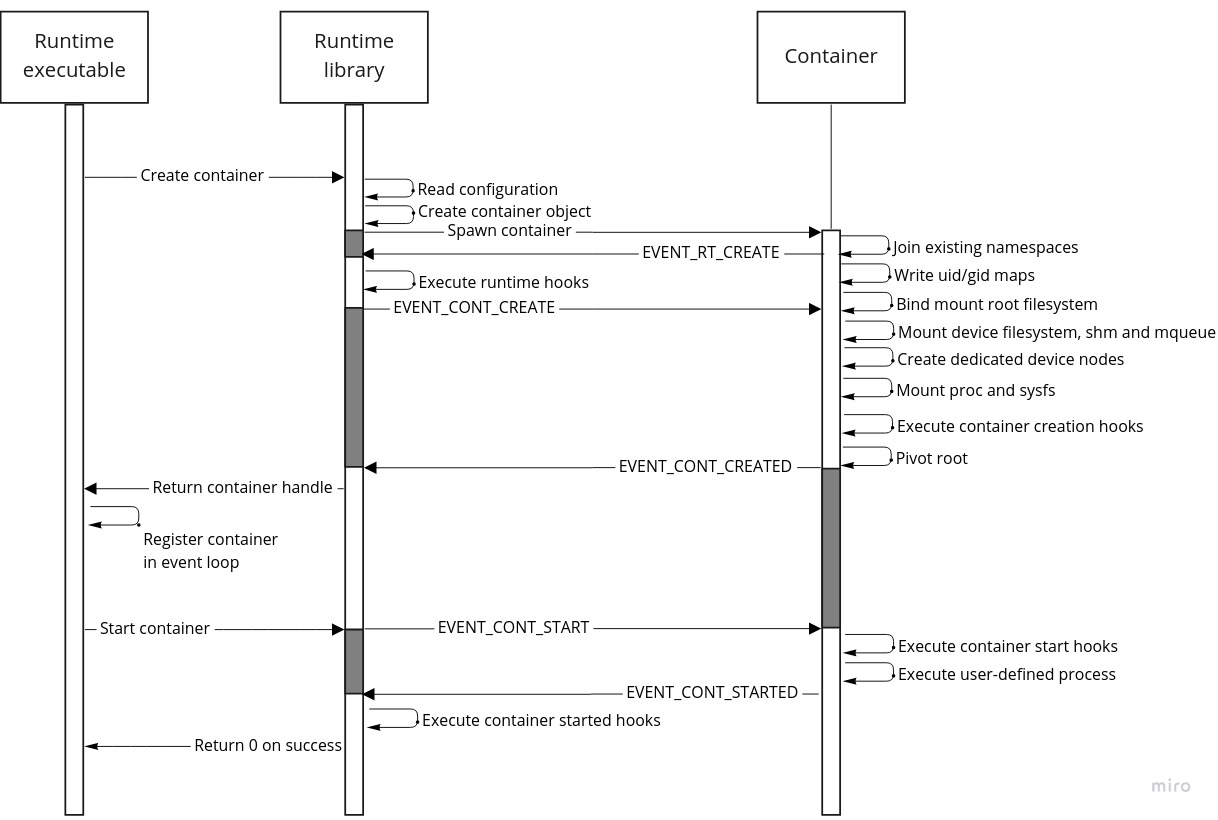
\includegraphics[width=0.8\textwidth]{images/concept/container-create-start-sequence-diagram.jpg}
    \caption{Sequence diagram highlighting the container creation and start operations}
    \label{images:concept/container-create-start-sequence-diagram.jpg}
\end{figure}

 The \verb|on_runtime_create| hooks are executed in the runtime namespace 
and prepare the runtime environment on the host. These hooks are triggered after the container process 
is cloned into a new set of namespaces. The \verb|on_container_created| hooks are executed within 
the container namespaces in order to prepare the runtime environment inside the container.
Note that these hooks are executed before the root filesystem is pivoted.
The \verb|on_container_start| hooks are triggered after pivoting the root filesystem, but before 
loading the user-defined application via \verb|execve()|. The \verb|on_container_started| hooks 
are executed within the runtime namespaces after the \verb|execve()| is called. 
The process is then monitored for state changes. Whenever it exits, the \verb|on_container_stopped|
hooks are executed, whose primary task is to clean up the runtime environment on the host. 

The synchronisation component defines an inter-process communication mechanism between 
the container runtime and a container. The typical communication flow follows the request-response pattern - 
one end produces a request and blocks until the other end consumes it and produces a response.
However, to enable concurrent work, a peer can \enquote{fire} a message and forget about the response.
The requests and responses are simple numeric values with semantic meaning. 

The container component brings all of the core components together. The sequence diagram in 
Figure \ref{images:concept/container-create-start-sequence-diagram.jpg} shows the procedures 
executed to create and start a container. The runtime executable invokes the create
operation, as defined in requirement (\ref{requirements:container-runtime/2}). 
The container component reads the configuration file and allocates 
an in-memory representation for the container. It then spawns the container process, which creates 
a freshly-allocated set of namespaces and joins already existing namespaces, depending on the namespace configuration 
specified in the file.

It then transitions into the \enquote{creating} state and notifies the runtime to execute the 
corresponding hooks by sending an \verb|EVENT_RT_CREATE| through the synchronisation component. 
The runtime receives the request, executes the runtime hooks, and notifies the child that it should transition 
into the \enquote{created} state by executing the container creation hooks and atomically swapping the old root mount 
with the new root filesystem. The container process then blocks indefinitely until it is killed 
or it receives a start request from the runtime executable. The latter will trigger yet another 
hook execution procedure, it will move the container into the \enquote{running} state and will afterwards run the user-defined binary. 
This is detected 
by the runtime, a set of post-start hooks is triggered, and the runtime executable is notified 
of the operation's completion.  

After the container is created, the executable is responsible for 
managing the container process. It does so by registering the container with an event loop that
polls container states and reaps processes that have terminated, which happens when the container 
transitions into the \enquote{stopped} state - either by exiting or being manually killed by the executable through 
a signal. 

%\begin{figure}[H]
%    \centering
%    \includegraphics[width=0.7\textwidth]{images/concept/runtime-create-start-kill-sequence-diagram.jpg}
%    \caption{Sequence diagram highlighting the interaction of a client application with the runtime executable.}
%    \label{images:concept/images/concept/runtime-create-start-kill-sequence-diagram.jpg}
%\end{figure}

%Figure \ref{images:concept/images/concept/runtime-create-start-kill-sequence-diagram.jpg} shows 
%the commands that an external application can send to the runtime executable. The application 
%creates a streaming socket and establishes a connection to the runtime server. 
%The runtime accepts the connection and registers the socket file descriptor with the event loop. 
%Whenever the client writes data into the socket, the runtime wakes up from the suspended state and reacts to the 
%event by parsing the request and processing it. When the client requests the creation 
%of a new container, by sending \verb|create <container-name> <config-path>|, 
%the runtime calls out to the library and registers the container in a hash table. Furthermore, 
%a pollable file descriptor for that container is created and registered with the event loop. 
%When the process exits, the kernel notifies the runtime of the event, so it can reap the process accordingly.
%The runtime is responsible for keeping the container's state machine consistent with the events 
%received from the kernel, as well as the requests that come from the client.

%The runtime uses the \verb|epoll| family of system calls to simultaneously monitor multiple file descriptors 
%to see if any I/O is possible on any of them. It also uses a new kernel application programming interface - 
%process file descriptors, commonly abbreviated as \verb|pidfd|'s, to map process identifiers to 
%pollable objects that can be registered with an event loop. All of these concepts are explained 
%in Chapter \ref{ch:implementation}.

\section{Benchmark}
Benchmarking is a tool to test performance in a controlled way, allowing different 
system and software configurations to be compared and analysed.

\subsection{Functional requirements}
\begin{enumerate}[i]
    \item The benchmark must facilitate the collection of performance metrics in native and containerised environments.
    \label{requirements:functional/benchmark/1} 
    \item The benchmark must aggregate and compare metrics in native and containerised environments to 
    enable the detection of isolation overheads.
    \label{requirements:functional/benchmark/2}
    \item The benchmark must produce observable results, either through visualisations or formatted text outputs,
    so that they can be analysed.
    \label{requirements:functional/benchmark/3}
    \item The benchmark must expose a command-line interface that allows users to define their own 
    container and sampling configurations.
    \label{requirements:functional/benchmark/4}
\end{enumerate}

\subsection{Workloads \& Metrics}
A workload is an application aimed at stressing a particular path of execution. 
Workloads are executed within an environment, e.g a container or on the host.
While the workload is running, a set of tracepoints accumulate performance counters relevant to that 
path of execution, which are then aggregated into statistics. 
The tracing procedures may be embedded in the workload itself, or as an external application. 

The tracepoints focus on building accurate representations of two variables - latency and throughput. 
The former is a measure of the time spent waiting for a particular resource. The latter 
is a measure of the number of operations than a resource can process per unit of time.
The benchmark tool, or the workload itself, attaches tracepoints to resources 
that are namespaced by the kernel and gathers information while the workload is running inside 
the container. Afterwards, the same statistics are gathered by executing the workload again, but this time 
as a native application absent of a noninterference boundary constructed by the container runtime. 
The difference in latency and throughput between both runs acts as an approximation of the isolation 
overhead introduced by sandboxing the workload. In Chapter \ref{ch:Experiment}, this approximation will be used 
to evaluate a set of hypotheses. 

In this section, the workloads and the performance counters associated with them are described. 

\subsubsection{Network workload}
The goal of this workload is to measure the overhead of data transmission between 
two separate network namespaces. The workload consists of a client and a server that communicate 
via TCP or UDP. Users have to specify the execution environment of both the client 
and the server. Hence, both can be deployed in two separate containers, each having a dedicated
virtual ethernet cable attached to a bridge device on the host that switches packets between them.
Alternatively, one of the components can run 
in the root network namespace, i.e directly on the host system. A third option is to have both 
the client and the server run on the host system without a bridge device between them. This is how 
native applications communicate - by being attached to the same network interface. 

The workload begins by starting the server and then the client. The client begins sending out as many 
data chunks of size $b$ as possible during equally-spaced intervals of $n$ seconds for a total 
duration of $t$ seconds.
During the data exchange procedure, the client keeps track of round-trip time, the number 
of bytes transfered, the bits transferred per second, and the number of retransmissions for each interval $n$. 
The caller configures $b$, $n$ and $t$. In additon, the caller is allowed to configure the number 
of parallel connections betwen the client and the server. In that case, the aforementioned 
statistics will be tracked for each connection. Increasing the number of connections can be used to
determine the degree of saturation, i.e how many connection are necessary to 
observe increases in latency and decreases in throughput due to throttling.
The workload also keeps a summary of the total user and system time it spends on the processing units,
both for the client and the server.

Note that the number of retransmissions and the round-trip time are metrics that are tracked only 
for TCP because they are intrinsic to the protocol implementation in order to detect data loss 
and retransmit packets accordingly. Conversely, UDP is unreliable and does not maintain such information. 
Lost data and out of order packets must be handled at the application level.

Round-trip time is this workload's latency metric. 
It is an approximation of the amount of time it takes to send a packet 
to the server plus the time it takes to receive the acknowledgement of that packet. 
The round-trip time is a value maintained by the kernel's TCP implementation.
The number of bytes transferred during the interval is this workload's throughput metric.
It shows how much data can be forwarded from one network namespace to another via the bridge
and its slave devices. This value is accumulated in user-space, whenever the \verb|read()| system call 
finishes on the receiver's end the counter is incremented.
The number of retransmissions acts as a robustness metric for the network itself.
It also has a statistical relationship with throughput.
Higher retransmission counts may have a negative impact on throughput.

\subsubsection{Filesystem workload}
The purpose of this workload is to detect and analyse differences in latency and throughput in 
different mount namespaces. In particular, we want to compare these metrics when running the 
workload within the root mount namespace and a container mount namespace. 

The workload executes operations on a single file. Users can define the I/O pattern issued to the file,
e.g performing only sequential reads, writing to the file at random file offsets, using direct I/O
in order to bypass the page cache and so on. In addition, the size of the buffers (the block size)
can be configured. How the workload should issue the I/O operations must also be specified. 
There are a plethora of options here. I/O operations can be synchronous, i.e employing calls to 
\verb|read()|, \verb|write()| and \verb|lseek()| to 
position file offsets. Alternatively, I/O operations can be asynchronous. That is, 
the workload registers a set of event handlers for each I/O operation it wants to execute and only 
submits requests to the kernel. The kernel does not block the calling thread. Instead,
it notifies the application whenever the disk driver emits an interrupt that represents 
the operation's completion. In asynchronous mode, users can configure the number of parallel 
I/O operations. Another way of controlling parallelisation is by spawning multiple processes that 
compete with each other. The number of processes is also configurable.

Input-output operations per second (IOPS) is this workload's throughput metric.
The metric is heavily dependant on the I/O pattern employed. 
This work focuses on sequential reads and writes, both in synchronous and asynchronous contexts.
For the asynchronous measurements, the number of in-flight I/O operations is controlled by 
two mechanisms - number of processes issuing I/O operations and number of parallel I/O operations 
by a single process. These mechanisms are used independently to ease the interpretation of the results.
For the synchronous measurements, the level of parallelisation is controlled only through the number 
of processes.

Total latency is this workload's latency metric. The total latency is derived by summing 
two variables - the submission latency and the completion latency. The former represents 
the time it takes to allocate and initialise the data buffers plus a variable $a$ whose interpretation 
depends on whether or not the underlying I/O mechanism is synchronous or not.  
If it is, then $a = 0$. Otherwise, $a$ includes the time it takes to submit the I/O operation
to the underlying queue of requests. The completion latency is also context-dependant. 
In the synchronous case, it represents the time from when the input-output operation was submitted 
to the kernel to when it was completed. In the asynchronous case, it is the time from 
when the submission operation was completed to when the event handler that reaps the operation 
was completed. Intuitively, synchronous operations exhibit lower submission latencies but higher 
completion latencies. Conversely, asynchronous operations exhibit higher submission latencies 
but lower completion latencies. Completion latencies have a stronger impact on overall 
I/O performance, making asynchronous mechanisms more favorable for performance-critical workloads.   

\subsubsection{Processing workload}
